\documentclass[a4paper]{article}
\usepackage[]{graphicx}\usepackage[]{color}
% maxwidth is the original width if it is less than linewidth
% otherwise use linewidth (to make sure the graphics do not exceed the margin)
\makeatletter
\def\maxwidth{ %
  \ifdim\Gin@nat@width>\linewidth
    \linewidth
  \else
    \Gin@nat@width
  \fi
}
\makeatother

\definecolor{fgcolor}{rgb}{0.345, 0.345, 0.345}
\newcommand{\hlnum}[1]{\textcolor[rgb]{0.686,0.059,0.569}{#1}}%
\newcommand{\hlstr}[1]{\textcolor[rgb]{0.192,0.494,0.8}{#1}}%
\newcommand{\hlcom}[1]{\textcolor[rgb]{0.678,0.584,0.686}{\textit{#1}}}%
\newcommand{\hlopt}[1]{\textcolor[rgb]{0,0,0}{#1}}%
\newcommand{\hlstd}[1]{\textcolor[rgb]{0.345,0.345,0.345}{#1}}%
\newcommand{\hlkwa}[1]{\textcolor[rgb]{0.161,0.373,0.58}{\textbf{#1}}}%
\newcommand{\hlkwb}[1]{\textcolor[rgb]{0.69,0.353,0.396}{#1}}%
\newcommand{\hlkwc}[1]{\textcolor[rgb]{0.333,0.667,0.333}{#1}}%
\newcommand{\hlkwd}[1]{\textcolor[rgb]{0.737,0.353,0.396}{\textbf{#1}}}%
\let\hlipl\hlkwb

\usepackage{framed}
\makeatletter
\newenvironment{kframe}{%
 \def\at@end@of@kframe{}%
 \ifinner\ifhmode%
  \def\at@end@of@kframe{\end{minipage}}%
  \begin{minipage}{\columnwidth}%
 \fi\fi%
 \def\FrameCommand##1{\hskip\@totalleftmargin \hskip-\fboxsep
 \colorbox{shadecolor}{##1}\hskip-\fboxsep
     % There is no \\@totalrightmargin, so:
     \hskip-\linewidth \hskip-\@totalleftmargin \hskip\columnwidth}%
 \MakeFramed {\advance\hsize-\width
   \@totalleftmargin\z@ \linewidth\hsize
   \@setminipage}}%
 {\par\unskip\endMakeFramed%
 \at@end@of@kframe}
\makeatother

\definecolor{shadecolor}{rgb}{.97, .97, .97}
\definecolor{messagecolor}{rgb}{0, 0, 0}
\definecolor{warningcolor}{rgb}{1, 0, 1}
\definecolor{errorcolor}{rgb}{1, 0, 0}
\newenvironment{knitrout}{}{} % an empty environment to be redefined in TeX

\usepackage{alltt}
\newcommand{\SweaveOpts}[1]{}  % do not interfere with LaTeX
\newcommand{\SweaveInput}[1]{} % because they are not real TeX commands
\newcommand{\Sexpr}[1]{}       % will only be parsed by R




\usepackage[utf8]{inputenc}
%\usepackage[ngerman]{babel}
\usepackage{a4wide,paralist}
\usepackage{amsmath, amssymb, xfrac, amsthm}
\usepackage{dsfont}
\usepackage[usenames,dvipsnames]{xcolor}
\usepackage{amsfonts}
\usepackage{graphicx}
\usepackage{caption}
\usepackage{subcaption}
\usepackage{framed}
\usepackage{multirow}
\usepackage{bytefield}
\usepackage{csquotes}
\usepackage[breakable, theorems, skins]{tcolorbox}
\usepackage{hyperref}
\usepackage{cancel}
\usepackage{bm}


% basic latex stuff
\newcommand{\pkg}[1]{{\fontseries{b}\selectfont #1}} % fontstyle for R packages

% Often used in exercise Rnw files, still relevant?
\newcommand{\lz}{\vspace{0.5cm}} % vertical space
\newcommand{\dlz}{\vspace{1cm}}  % double vertical space

% Unused and about to be deleted
\newcommand{\oneliner}[1] % Oneliner for important statements
{\begin{block}{}\begin{center}\begin{Large}#1\end{Large}\end{center}\end{block}}


%--------------------%
%  New environments  %
%--------------------%

 % Frame with breaks and verbatim // this is used very often
\newenvironment{vbframe}
{
\begin{frame}[containsverbatim,allowframebreaks]
}
{
\end{frame}
}

% Frame with verbatim without breaks (to avoid numbering one slided frames)
% This is not used anywhere but I can see it being useful
\newenvironment{vframe}
{
\begin{frame}[containsverbatim]
}
{
\end{frame}
}

% Itemize block
\newenvironment{blocki}[1]
{
\begin{block}{#1}\begin{itemize}
}
{
\end{itemize}\end{block}
}

%--------------%
%  Citebutton  %
%--------------%
% Example usage (from slides-cart-discussion.tex)
% \citebutton{Breiman, 1984}{https://www.taylorfrancis.com/books/mono/10.1201/9781315139470/classification-regression-trees-leo-breiman}
\newcommand{\citebutton}[2]{%
\NoCaseChange{\resizebox{!}{9pt}{\protect\beamergotobutton{\href{#2}{#1}}}}%
}

% textcolor that works in mathmode
% https://tex.stackexchange.com/a/261480
% Used e.g. in forests/slides-forests-bagging.tex
% [...] \textcolor{blue}{\tfrac{1}{M}\sum^M_{m} [...]
\makeatletter
\renewcommand*{\@textcolor}[3]{%
  \protect\leavevmode
  \begingroup
    \color#1{#2}#3%
  \endgroup
}
\makeatother


\tcbset{enhanced}

\DeclareRobustCommand{\mybox}[2][gray!20]{%
	\iffalse
	\begin{tcolorbox}[   %% Adjust the following parameters at will.
		breakable,
		left=0pt,
		right=0pt,
		top=0pt,
		bottom=0pt,
		colback=#1,
		colframe=#1,
		width=\dimexpr\linewidth\relax,
		enlarge left by=0mm,
		boxsep=5pt,
		arc=0pt,outer arc=0pt,
		]
		#2
	\end{tcolorbox}
	\fi
}

\DeclareRobustCommand{\myboxshow}[2][gray!20]{%
%	\iffalse
	\begin{tcolorbox}[   %% Adjust the following parameters at will.
		breakable,
		left=0pt,
		right=0pt,
		top=0pt,
		bottom=0pt,
		colback=#1,
		colframe=#1,
		width=\dimexpr\linewidth\relax,
		enlarge left by=0mm,
		boxsep=5pt,
		arc=0pt,outer arc=0pt,
		]
		#2
	\end{tcolorbox}
%	\fi
}


%exercise numbering
\renewcommand{\theenumi}{(\alph{enumi})}
\renewcommand{\theenumii}{\roman{enumii}}
\renewcommand\labelenumi{\theenumi}


\font \sfbold=cmssbx10

\setlength{\oddsidemargin}{0cm} \setlength{\textwidth}{16cm}


\sloppy
\parindent0em
\parskip0.5em
\topmargin-2.3 cm
\textheight25cm
\textwidth17.5cm
\oddsidemargin-0.8cm
\pagestyle{empty}

\newcommand{\kopf}[1] {
\hrule
\vspace{.15cm}
\begin{minipage}{\textwidth}
%akwardly i had to put \" here to make it compile correctly
	{\sf\bf Introduction to Machine Learning \hfill Exercise sheet #1\\
	 \url{https://introduction-to-machine-learning.netlify.app/} \hfill WiSe 2020/2021}
\end{minipage}
\vspace{.05cm}
\hrule
\vspace{1cm}}

\newenvironment{allgemein}
	{\noindent}{\vspace{1cm}}

\newcounter{aufg}
\newenvironment{aufgabe}
	{\refstepcounter{aufg}\textbf{Exercise \arabic{aufg}:}\\ \noindent}
	{\vspace{0.5cm}}

\newcounter{loes}
\newenvironment{loesung}
	{\refstepcounter{loes}\textbf{Solution \arabic{loes}:}\\\noindent}
	{\bigskip}
	
\newenvironment{bonusaufgabe}
	{\refstepcounter{aufg}\textbf{Exercise \arabic{aufg}*\footnote{This
	is a bonus exercise.}:}\\ \noindent}
	{\vspace{0.5cm}}

\newenvironment{bonusloesung}
	{\refstepcounter{loes}\textbf{Solution \arabic{loes}*:}\\\noindent}
	{\bigskip}



\begin{document}
% !Rnw weave = knitr




\kopf{5}


\loesung{

\begin{enumerate}
  \item[a)] First, sort the table:
  \begin{center}
  \begin{tabular}{ | c | c | c | c |}
  \hline
  ID & Actual Class & Score & Predicted Class \\ \hline
  6 & 0 & 0.63 & 1  \\
  7 & 1 & 0.62 & 1  \\
  10 & 0 & 0.57 & 1 \\
  \hline
  4 & 1 & 0.38 & 0  \\
  1 & 0 & 0.33 & 0  \\
  8 & 1 & 0.33 & 0  \\
  2 & 0 & 0.27 & 0  \\
  5 & 1 & 0.17 & 0  \\
  9 & 0 & 0.15 & 0 \\
  3 & 1 & 0.11 & 0  \\
  \hline\text{
  }  \end{tabular}
  \end{center}


  \begin{center}
  \begin{tabular}{ | c | c | c | }
  \hline
   & Actual Class - 0 & Actual Class - 1  \\
  Prediction - 0 & 3 & 4  \\
  Prediction - 1 & 2 & 1  \\
      \hline
    \end{tabular}
  \end{center}

  so we get

  \begin{center}
  \begin{tabular}{ | c | c | c | c | }
  \hline
  FN & FP & TN & TP   \\ \hline
  4 & 2 & 3 & 1 \\
      \hline
    \end{tabular}
  \end{center}

  \item[b)]

  $$\text{Precision} = \frac{\text{TP}}{\text{TP} + \text{FP}} =\frac{1}{3} $$

  $$\text{Sensitivity} = \frac{\text{TP}}{\text{TP} + \text{FN}} =\frac{1}{5} $$

  $$\text{Accuracy} = \frac{\text{TP} + \text{TN}}{\text{TP} + \text{TN} + \text{FP} + \text{FN}} =\frac{4}{10} $$

  $$\text{Specificity}  = \frac{\text{TN}}{\text{TN} + \text{FP}} =\frac{3}{5} $$

  $$\text{Error Rate}  = \frac{\text{FP} + \text{FN}}{\text{TP} + \text{TN} + \text{FP} + \text{FN}} =\frac{6}{10} $$

  $$\text{F-measure} = \frac{2\cdot\text{Precision}\cdot\text{Sensitivity}}{\text{Precision}+\text{Sensitivity}} = 0.25 $$

  $$\text{Negative Predictive Value} = \frac{\text{TN}}{\text{TN} + \text{FN}} =\frac{3}{7} $$

  \item[c)] 
First we sort the results by the score: \\
\begin{knitrout}
\definecolor{shadecolor}{rgb}{0.969, 0.969, 0.969}\color{fgcolor}
\begin{tabular}{l|r|r}
\hline
  & true\_labels & scores\\
\hline
6 & 0 & 0.63\\
\hline
7 & 1 & 0.62\\
\hline
10 & 0 & 0.57\\
\hline
4 & 1 & 0.38\\
\hline
1 & 0 & 0.33\\
\hline
8 & 1 & 0.33\\
\hline
2 & 0 & 0.27\\
\hline
5 & 1 & 0.17\\
\hline
9 & 0 & 0.15\\
\hline
3 & 1 & 0.10\\
\hline
\end{tabular}

\end{knitrout}
Here we see that $\frac{1}{n_+} = \frac{1}{5} = 0.2$ and $\frac{1}{n_-} = \frac{1}{5} = 0.2$. Now we follow the algorithm as described in the lecture slides:
\begin{enumerate}
\item Set $\alpha = 1$, so we start in $(0,0)$; we predict everything as 1.
\item Set threshold $\tau = 0.625$ yields TPR 0 and FPR  $0 + \frac{1}{n_-} = 0.2$. (Obs. 6 is "0")
\item Set threshold $\tau = 0.6$ yields TPR $0 + \frac{1}{n_+} = 0.2$ and FPR  $0.2$. (Obs. 7 is "1")
\item Set threshold $\tau = 0.5$ yields TPR 0.2 and FPR  $0.2 + \frac{1}{n_-} = 0.4$. (Obs. 10 is "0")
\item Set threshold $\tau = 0.35$ yields TPR $0.2 + \frac{1}{n_+} = 0.4$ and FPR  $0.4$. (Obs. 4 is "1")
\item Set threshold $\tau = 0.3$ yields TPR $0.4 + \frac{1}{n_+} = 0.6$ and FPR  $0.4 + \frac{1}{n_-} = 0.6$. (Obs. 1/8 is "0"/"1")
\item Set threshold $\tau = 0.2$ yields TPR $0.6$ and FPR  $0.6 + \frac{1}{n_-} = 0.8$. (Obs. 2 is "0")
\item Set threshold $\tau = 0.16$ yields TPR $0.6 + \frac{1}{n_+} = 0.8$ and FPR  $0.8$. (Obs. 5 is "1")
\item Set threshold $\tau = 0.14$ yields TPR $0.8$ and FPR  $0.8 + \frac{1}{n_-} = 1$. (Obs. 9 is "0")
\item Set threshold $\tau = 0.09$ yields TPR $0.8 + \frac{1}{n_+} = 1$ and FPR  $1$. (Obs. 3 is "1")
\end{enumerate}

Therefore we get the polygonal path consisting of the ordered list of vertices \[(0,0), (0.2,0), (0.2,0.2),
(0.4,0.2), (0.4,0.4), (0.6,0.6), (0.8,0.6), (0.8, 0.8), (1, 0.8), (1,1).\]

\begin{knitrout}
\definecolor{shadecolor}{rgb}{0.969, 0.969, 0.969}\color{fgcolor}\begin{kframe}
\begin{alltt}
\hlkwd{library}\hlstd{(ggplot2)}
\hlstd{roc_data} \hlkwb{<-} \hlkwd{data.frame}\hlstd{(}\hlkwc{TPR} \hlstd{=} \hlkwd{c}\hlstd{(}\hlnum{0}\hlstd{,} \hlnum{0}\hlstd{,}   \hlnum{0.2}\hlstd{,} \hlnum{0.2}\hlstd{,} \hlnum{0.4}\hlstd{,} \hlnum{0.6}\hlstd{,} \hlnum{0.6}\hlstd{,} \hlnum{0.8}\hlstd{,} \hlnum{0.8}\hlstd{,} \hlnum{1}\hlstd{),}
                       \hlkwc{FPR} \hlstd{=} \hlkwd{c}\hlstd{(}\hlnum{0}\hlstd{,} \hlnum{0.2}\hlstd{,} \hlnum{0.2}\hlstd{,} \hlnum{0.4}\hlstd{,} \hlnum{0.4}\hlstd{,} \hlnum{0.6}\hlstd{,} \hlnum{0.8}\hlstd{,} \hlnum{0.8}\hlstd{,}  \hlnum{1}\hlstd{,}  \hlnum{1}\hlstd{))}

\hlkwd{ggplot}\hlstd{(roc_data,} \hlkwd{aes}\hlstd{(}\hlkwc{x} \hlstd{= FPR,} \hlkwc{y} \hlstd{= TPR))} \hlopt{+} \hlkwd{geom_line}\hlstd{()} \hlopt{+}
  \hlkwd{geom_abline}\hlstd{(}\hlkwc{slope} \hlstd{=} \hlnum{1}\hlstd{,} \hlkwc{intercept} \hlstd{=} \hlnum{0}\hlstd{,} \hlkwc{linetype} \hlstd{=} \hlstr{'dashed'}\hlstd{)}
\end{alltt}
\end{kframe}

{\centering 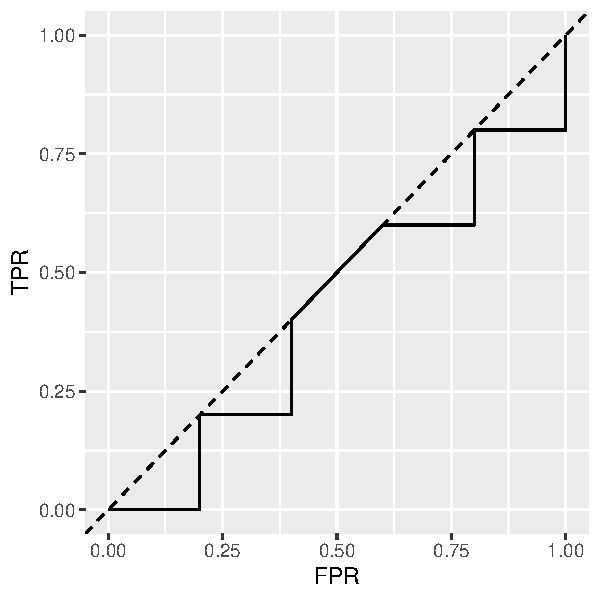
\includegraphics[width=\maxwidth]{figure/unnamed-chunk-3-1} 

}


\end{knitrout}

We see that the resulting ROC lies below the line from the origin with a slope of 1, which represents
a random classifier, i.e., the scoring algorithm performs worse than a random classifier.
If this happens while evaluating the training data, the labels of the scoring algorithm should be inverted.

  \item[d)] 
  We can compute the AUC (\textit{area under the curve}) by looking at the ROC, s.t.
  $$
  AUC = 0.5 - 4 \cdot (0.2 \cdot 0.2 \cdot 0.5) = 0.42.
  $$

\end{enumerate}
}
\end{document}
